\chapter{Verfahrensbeschreibung}\label{ch:verfahrensbeschreibung}


\section{Gesamtsystem}\label{ver:sec:gesamtsystem}
Das System arbeitet nach dem EVA-Prinzpip. Die EVA-Segmente werden von einem Controller erweitert, welcher das Programm koordiniert und den Einstiegspunkt des Programms darstellt.

\subsection{Eingabe}\label{ver:subsec:eingabe}
Um ein vollständiges Bahnnetz abbilden zu können werden alle Bahnverbindungen aus der Eingabedatei eingelesen. Dafür werden die einzelnen Stationen einer Verbindung als \texttt{String} in eine \texttt{ArrayListe} gespeichert. Diese Listen lassen sich dann in ein Objekt Objekt Zugverbindung (siehe \ref{ver:subsubsec:trainconnection}) umwandeln. Die erstellten \texttt{TrainConnection}-Objekte werden in einer Liste gesammelt und nach einlesen der Datei dem Controller übergeben.\\

\subsection{Verarbeitung}\label{subsec:verarbeitung}
Die Liste mit den Zugverbindungen kann nun weiterverarbeitet werden. Dafür wird diese in ein Objekt \texttt{TrainWeb}(\ref{ver:subsubsec:trainweb}) umgewandelt welches Hauptbestandteil der Datenspeicherung ist.\\
Vor der eigentlichen Berechnung des Algorithmus wird das Netzt nun noch reduziert. Dafür wird dieses einem \texttt{Reducer}(\ref{ver:subsubsec:reducer}) übergeben, der die Verbindungen und die darin enthaltenen Staionen in eine minimale aber informationsidentische Form reduziert. \\
Nach der Reduktion wird das reduzierte Netz an den Algorithmus übergeben. Dieser ermittelt nun die minimale Anzahl an Servicestationen und deren Standorte. Die Standorte werden als \texttt{Station}(\ref{ver:subsubsec:station}) in einer \texttt{ArrayList} zurück an den Controller übergeben\\

\subsection{Ausgabe}\label{ver:subsec:ausgabe}
Die ermittelte Liste wird nun an die Ausgabe weitergegeben. Diese nimmt die Liste mit den ermittelten Stationen entgegen und schreibt diese in eine Ausgabedatei.\\

\section{Datenstrukturen}\label{ver:subsec:datenstrukturen}
Um die Verarbeitung der Daten übersichtlich zu gestalten werden verschiedene Datenstrukturen erstellt. Dabei lässt sich unterscheiden in Speicher Strukturen und Verarbeitungsstrukturen.\\
\subsection{Speicherstrukturen}\label{ver:subsec:Speicherstrukturen}
Alle erstellten Datenstrukturen basieren auf ArrayListen. Diese bieten einerseits eine dynamische Speichermöglichkeit. Andererseits ermöglicht dies ein optimale Speicherung, da durch die Nutzung von ArrayListen die Zugnetzdaten nur einmal gespeichert und dann als Referenzen weitergegeben werden können. Dies verhindert unnötiges Kopieren und erleichtert Vergleiche.\\

\subsubsection{TrainConnection}\label{ver:subsubsec:trainconnection}
Hauptbestandteil der Datenvermittlung ist die Klasse \texttt{TrainConnection}. Diese besitzt als einziges Attribut eine \texttt{ArrayList} in welcher Stationen als String abgespeichert werden. Diese Stationen bilden dann eine vollständige  Zugverbindung ab.

Außerdem sind zwei Vergleichmethoden implementiert. Diese ermöglichen die gespeicherte Liste an Stationen, von zwei Objekten TrainConnection
 miteinander zu vergleichen. Eine Methode vergleicht die Anzahl der Stationen (hat die Verbindung mehr Haltestellen als die andere?). Die zweite Methode überprüft den Inhalt der Stationen (fahren beide Verbindungen die gleichen Stationen an?)\\

\subsubsection{Station}\label{ver:subsubsec:station}
Um im Verlaufe der Verfahren strukturiert vorgehen zu können existiert die Klasse \texttt{Station}. Diese speichert den Namen einer Station als \texttt{String} und eine \texttt{ArrayListe} mit Bahnverbindungen(\ref{ver:subsubsec:trainconnection}) in der der die Station angefahren wird.

Wie in \ref{ver:fig:datenstruktur_zusammenhaenge} zu sehen, werden dabei keine Kopien der \texttt{TrainConnection}'s erstellt sondern nur Referenzen auf die ursprünglichen Objekte gespeichert.

Diese Klasse ist dabei nur eine Hilfestellung für spätere Operationen. Die eigentlichen Bahnstationen werden weiterhin als \texttt{String} gespeichert und verglichen. Durch diese Klasse wird verhindert, jedesmal alle Bahnverbindungen zu ermitteln zu müssen in denen eine Station vorkommt.\\

\subsubsection{TrainWeb}\label{ver:subsubsec:trainweb}
Mit diesen beiden Speicherstrukturen lässt sich nun das gesamte Bahnnetz übersichtlich speichern. Dafür stehen in dem Objekt \texttt{TrainWeb} zwei Attribute zur Verfügung. Eine \texttt{ArrayListe} mit allen Bahnverbindungen(\ref{ver:subsubsec:trainconnection}) und eine \texttt{ArrayListe} mit allen Bahnstationen(\ref{ver:subsubsec:station}).

Dafür werden alle Verbindungen aus der eingelesen Datei direkt abgelegt. Die Bahnstationen können nun über das Iterieren aller Bahnverbindungen ermittelt werden. Für neue Stationen wird dann erneut über alle Verbindungen iteriert, um alle stationsbeinhaltende Verbindungen zusammen mit dem Stationsnamen als \texttt{Station}-Objekt (\ref{ver:subsubsec:station}) speichern zu können.\\

\begin{center}
    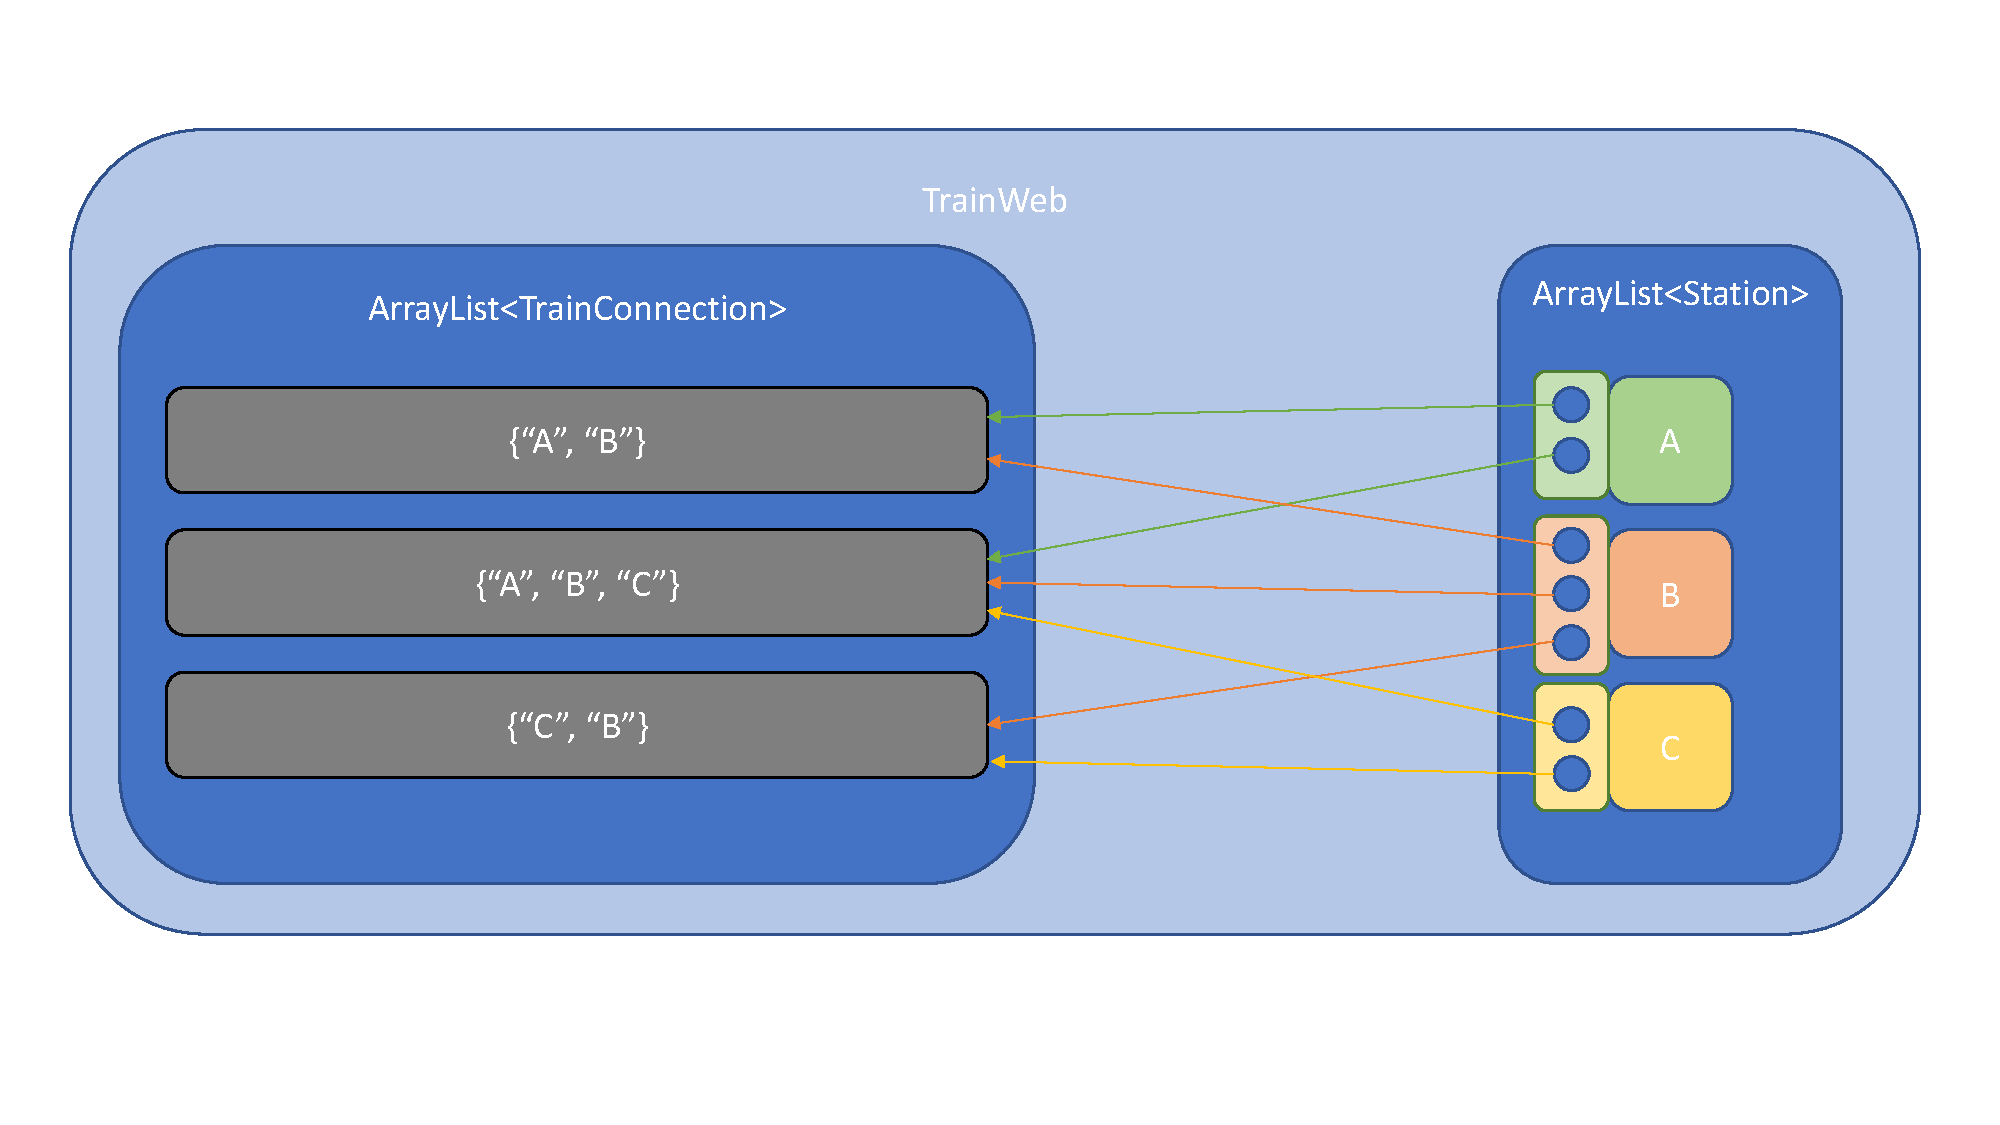
\includegraphics[width=\linewidth]{images/Datenstruktur_Zusammenhaenge.pdf}
    \captionof{figure}{Speicherstrukturen und ihre Zusammenhänge}
    \label{ver:fig:datenstruktur_zusammenhaenge}
\end{center}

\subsection{Verarbeitungsstrukturen}\label{ver:subsec:verarbeitungsstrukturen}
Die Verarbeitungsstrukturen nehmen nun einen fertigen Netzplan entgegen auf dem sie arbeiten.\\

\subsubsection{Reducer}\label{ver:subsubsec:reducer}
Der Reducer hat dabei keinen Rückgabewert. Dieser wendet die drei, als Methoden implementierten, Reduktionsverfahren(siehe \ref{ver:subsec:reduktionsverfahren}) direkt auf den Netzplan an.\\

\subsubsection{Algorithmus}\label{ver:subsubsec:algorithmus}
Der reduzierte Netzplan wird nun dem Algorithmus übergeben. Dieser ermittelt anhand des Plans, Bahnstationen um das gesamte Netz versorgen zu können.

\section{Verbale beschreibung der Verfahren}\label{ver:sec:verfahren}
\subsection{Berechnung der minimalen Anzahl an Servicestationen}\label{ver:subsec:berechnung}
Dieser wählt nun iterativ die Stationen aus, die die meisten Verbindungen abdecken. Diese werden dann in einer Liste gespeichert. Mit dieser Liste kann nun überprüft werden ob alle Stationen  Anschließend werden alle Verbindungen die von diesen Stationen abgedeckt werden aus dem Netzplan entfernt. Dieser Vorgang wird solange wiederholt bis alle Verbindungen abgedeckt sind.\\

\subsection{Beschreibung der drei Reduktionsverfahren}\label{ver:subsec:reduktionsverfahren}
\subsubsection{Doppelstationen}\label{ver:subsubsec:doppelstationen}
In diesem Verfahren werden alle Zugverbindungen nach Mehrfachvorkommen von Stationen geprüft. Sollte eine Station mehrfach in einer Verbindung angefahren werden, braucht diese nur einmal in der Zugverbindung gespeichert werden. Für die spätere Berechnung ist nur relevant welche Stationen in einer Zugverbindung angefahren werden. Die Reihenfolge der Stationen spielt somit keine Rolle. Somit gehen durch die einfache Speicherung von Stationen keine Inforamtionen verloren.\\

\subsubsection{Stationsabhängigkeiten}
In diesem Verfahren werden Stationsabhängigkeiten geprüft. Sollte in allen Zugverbindung die eine beliebige Station A beinhaltet, auch eine Station B angefahren werden kann die betrachtete Station A in allen Zugverbindungen entfernt werden. Es ist davon auszugehen, dass dabei kein Informationsverlust riskiert wird, da jede Zugverbindung der betrachteten Station A auch die gefundene Station B passieren wird. Die Menge der Zugverbindungen die Station A anfahren ist also eine Teilmenge der Verbindungen Station B und müssen nichtmehr gesondert gespeichert und überprüft werden. Dabei kann es dazu kommen, dass Zugverbindungen aus nurnoch einer Station bestehen.\\

\subsubsection{Implizite Zugverbindungen}
In diesem Verfahren wird überprüft ob eine Zugverbindung implizit in einer anderen Zugverbindung enthalten ist. Sollte dies der Fall sein, darf die größere Zugverbindung entfernt werden. Dies ist erlaubt, da alle Stationen der kleineren Verbindung auch in der größeren Verbindung angefahren werden. Eine Überprüfung der kleineren Zugverbindung ist also Ausreichend um beiden Verbindungen eine Servicestationen zu gewährleisten. Die größere Verbindung ist somit redundant.\\

